\documentclass{beamer}

\usepackage[utf8]{inputenc}

\usepackage[T1]{fontenc}
\usepackage{tikz}
\usepackage{babel,textcomp}

\usetheme{Ifi}
\setbeamertemplate{navigation symbols}{}

\date{Junio 2023}

\begin{document}

\begin{frame}{}
\end{frame}


\begin{frame}{Aspectos generales del artículo}
    \begin{itemize}


        \item Autora: Dian Savitri\\
        \item Presentado en: MISEIC(2019)\\
        \item Publicado en: Journal of Physics, Conference Series\\
        \item Factor de impacto: 0.227\\
        \item Factor de impacto de la revista: 0.21
    \end{itemize}
\end{frame}
\begin{frame}{Aspectos generales del artículo}
    \begin{itemize}
        \item {\bf Objetivo del artículo:} Analizar la estabilidad del modelo presa-depredador.\\

        \item {\bf Valoración del artículo:} Los autores consideramos que presenta varios errores, tanto tipográfico como de contenidos. Su factor de impacto es
              relativamente bajo. Sin embargo consideramos que se tratan temáticas muy interesantes y de gran utilidad para el desarrollo de la ecología.
    \end{itemize}

    % El modelo fue construido a partir de dos presas que involucran una estructura de etapa y un depredador. Posee tres equilibrios positivos: el original, la extinción del
    % depredador y un punto interior. El artículo hace un estudio de la dinámica
    % del comportamiento de las interacciones presa-depredador, con la función de respuesta Holling tipo II(esta respuesta funcional se
    % refiere al cambio en el comportamiento de los individuos en función de la densidad del huésped o presa) para presas adultas. El apartado considera la estabilidad de
    % los equilibrios en detalle con las condiciones de existencia e ilustra la estabilidad local de los equilibrios, además cuenta con simulaciones numéricas para ilustrar
    % los resultados.
\end{frame}

\begin{frame}{Estructura del trabajo}
    \begin{itemize}
        \item Modelo matemático
        \item Análisis de los puntos de equilibrio
        \item Simulaciones numéricas
    \end{itemize}
\end{frame}
\begin{frame}{Ecuaciones que ilustran el modelo utilizado}

    \begin{eqnarray*}
        \frac{dx}{dt} &=& rx(1-\frac{x}{k})-\beta x-\alpha xz\\
        \\
        \frac{dy}{dt} &=& \beta x-\frac{\eta yz}{y+m}-\mu y\\
        \\
        \frac{dz}{dt} &=& \alpha_1 xz+\rho z^2-\frac{\eta_1z^2}{y+m}
    \end{eqnarray*}
\end{frame}

\begin{frame}

    {\bf $$\frac{dx}{dt} = rx(1-\frac{x}{k})-\beta x-\alpha xz$$ }

    % El término $rx(1-\frac{x}{k})$ de (\ref*{dx}) es conocido como ecuación
    %           logística

    $x$: población de presas juveniles.

    $t$: tiempo.

    $r$: constante que define la tasa de crecimiento.

    $k$: capacidad de carga o persistencia

    % Esta primera ecuación representa el modelo de crecimiento poblacional en las
    % presas jóvenes. Para ello se tuvo en cuenta:
    % \begin{itemize}
    %     \item La tasa de reproducción es proporcional a la población existente.
    %     \item La tasa de reproducción es proporcional a la cantidad de recursos disponibles.
    %     \item La competición por los recursos disponibles tiende a limitar el crecimiento poblacional.
    % \end{itemize}
    % $\beta x$ representa las presas que se vuelven adultas.

    $\beta$: factor de conversión de presa joven a presa adulta

    %    La velocidad con que varía la población de presas $x$ es proporcional al número de encuentros con los depredadores $z$ según la ecuación de Lotka-Volterra:
    %     $$\frac{dx}{dt}=\alpha xz$$
    $\alpha$: tasa de eliminación de presas por parte de los depredadores.

\end{frame}

\begin{frame}
    {\bf $$\frac{dy}{dt} = \beta x-\frac{\eta yz}{y+m}-\mu y$$}
    % El primer término de la ecuación ya fue analizado anteriormente, es la cantidad de presas jóvenes que se convierten en adultas.
    % El proceso de eliminación de presas por los depredadores se describe a partir del modelo Holling Tipo II, que establece:

    $\eta$: valor máximo de la tasa de reducción per cápita de presas adultas debido a los depredadores.
    \vspace*{0.3cm}

    $m$: coeficiente de protección ambiental para las presas adultas.
    \vspace*{0.3cm}

    %   Además se considera las presas que mueren de forma natural $\mu y$.
    $\mu$: tasa de mortalidad en presas adultas.
\end{frame}

\begin{frame}
    {\bf $$\frac{dz}{dt} = \alpha_1 xz+\rho z^2-\frac{\eta_1z^2}{y+m}$$}

    % $\alpha_1 xz+\rho z^2$ representa el crecimiento según disponibilidad de alimentos favoritos de los depredadores.

    $\alpha_1$: tasa de disponibilidad de alimentos favoritos de los depredadores.

    $\rho$: tasa de crecimiento intrínseco.

    %  Además se considera que esta población decrece a partir del modelo de Leslie-Gower modificado:

    %   $$\frac{dz}{dt} =-\frac{\rho z^2}{n y+c}$$

    %   $$\frac{dz}{dt} =-\frac{\frac{\rho}{x} z^2}{y+\frac{c}{n}}$$

    %   $n$: calidad energética de la presa como alimento.

    %   $c$: tamaño máximo de disponibilidad de alimentos alternativos.

    %   $$\frac{\rho}{n}=\eta_1$$

    %   $$\frac{c}{n}=m$$
    $\eta_1$: relación del crecimiento intríseco y el factor de conversión de depredación a presa adulta.

    $m$: pérdida residual de los depredadores.
    \vspace*{0.7cm}

    {\it\scriptsize Aquí discrepamos. Consideramos que Savitri pudo tener un error tipográfico, pues en lo adelante asume nuestra
    ecuación, además [2] defiende este modelo.}

\end{frame}

\begin{frame}{Análisis de los puntos de equilibrio y su estabilidad}

    Los puntos de equilibrio para este sistema son aquellos que satisfacen:
    $$\frac{dx}{dt}=\frac{dy}{dt}=\frac{dz}{dt}=0$$

    Estos puntos son:
    \begin{itemize}
        \item $P_1=(0, 0, 0)$
        \item $P_2=(\frac{k(r-\beta)}{r}, \frac{\beta k(r-\beta)}{\mu r}, 0)$
        \item $P_3=(x_3, y_3, z_3)$
    \end{itemize}
\end{frame}

\begin{frame}
    {Matriz Jacobiana}
    $$\left(
        \begin{array}{ccc}
                r-\frac{2rx}{k}-\beta-\alpha z & 0                                       & -\alpha x                       \\
                \beta                          & \frac{-nz}{y+m}+\frac{nyz}{(y+m)^2}-\mu & \frac{-ny}{y+m}                 \\
                \alpha_1z                      & \frac{n_1z^2}{(y+m)^2}                  & 2pz-\frac{2n_1z}{y+m}+\alpha_1x
            \end{array}
        \right)$$
\end{frame}

\begin{frame}
    Para $P_1$ sería:
    $$\left|
        \begin{array}{ccc}
            (-\beta+r)-\lambda & 0      l     & 0        \\
            \beta              & -\mu-\lambda & 0        \\
            0                  & 0            & -\lambda
        \end{array}
        \right| =0$$

    $\lambda_1=-\beta+r$, $\lambda_2 = -\mu$ y $\lambda_3=0$

    {\bf Por tanto en $P_1$ el sistema es inestable.}
    \vspace*{0.7cm}

    {\it\scriptsize En este punto, Savitri se refiere a $-1+r$ donde nosotros a $-\beta+r$. Consideramos que haya sido un error tipográfico, pues como bien ella
        afirma, esta matriz se obtiene al sustituir el punto de equilibrio (0, 0, 0).}

\end{frame}

\begin{frame}
    Para $P_2$ sería:
    $$\left|
        \begin{array}{ccc}
            (\beta+r)-\lambda & 0            & \frac{\alpha k(\beta-r)}{r}                                      \\
            \beta             & -\mu-\lambda & \frac{n\beta k(\beta-r)}{r\mu (\frac{\beta k(r-\beta)}{r\mu}+m)} \\
            0                 & 0            & \frac{\alpha_1 k(\beta-r)}{r}-\lambda
        \end{array}
        \right| =0$$

    $\lambda_1=\beta-r, \lambda_2=-\mu, \lambda_3=-\frac{\alpha_1 k(\beta-r)}{r}$

    {\bf Por lo que $P_2$ es inestable.}
    \vspace*{0.7cm}

    {\it\scriptsize En la tercera fila, tercera columna, [1] olvida restar $\lambda$, asumimos error tipográfico}

    {\it\scriptsize [1] considera este punto estable, diferimos de su resultado}

\end{frame}
\begin{frame}

    En el caso de $P_3$:
    \vspace*{0.5cm}

    $J(x_3, y_3, z_3) =$
    $$
        \left(
        \begin{array}{ccc}
                r-\frac{2rx_3}{k}-\beta-\alpha z_3 & 0                                                 & -\alpha x_3                             \\
                \beta                              & \frac{-nz_3}{y_3+m}+\frac{ny_3z_3}{(y_3+m)^2}-\mu & \frac{-ny_3}{y_3+m}                     \\
                \alpha_1z_3                        & \frac{n_1z_3^2}{(y_3+m)^2}                        & 2pz_3-\frac{2n_1z_3}{y_3+m}+\alpha_1x_3
            \end{array}
        \right)$$
\end{frame}
\begin{frame}
    $$\lambda^3+\gamma_1\lambda^2+\gamma_2\lambda+\gamma_3=0 $$

    Estable $\leftrightarrow$ $\gamma_1>0, \gamma_3>0$ y $\gamma_1\gamma_2-\gamma_3>0$
    \vspace*{0.3cm}

    {\bf La coexistencia en $P_3$ es local y asintóticamente estable.}
    \vspace*{0.3cm}

    {\it \scriptsize Aquí [1] trabaja con $\lambda^2-\ traza\ \lambda+\ deteminante$, esto no es aplicable para sistemas mayores que dos, ni
    es resultado de simplificación alguna}
\end{frame}

\begin{frame}
    {Primer experimento}

    En el primer conjunto de experimentos se usaron los valores iniciales $[x_0=3.01, y_0=5.05, z_0=4.28]$
    y $[x_0=4.6, y_0=5.9, z_0=3.1]$

    \begin{figure}[h!]
        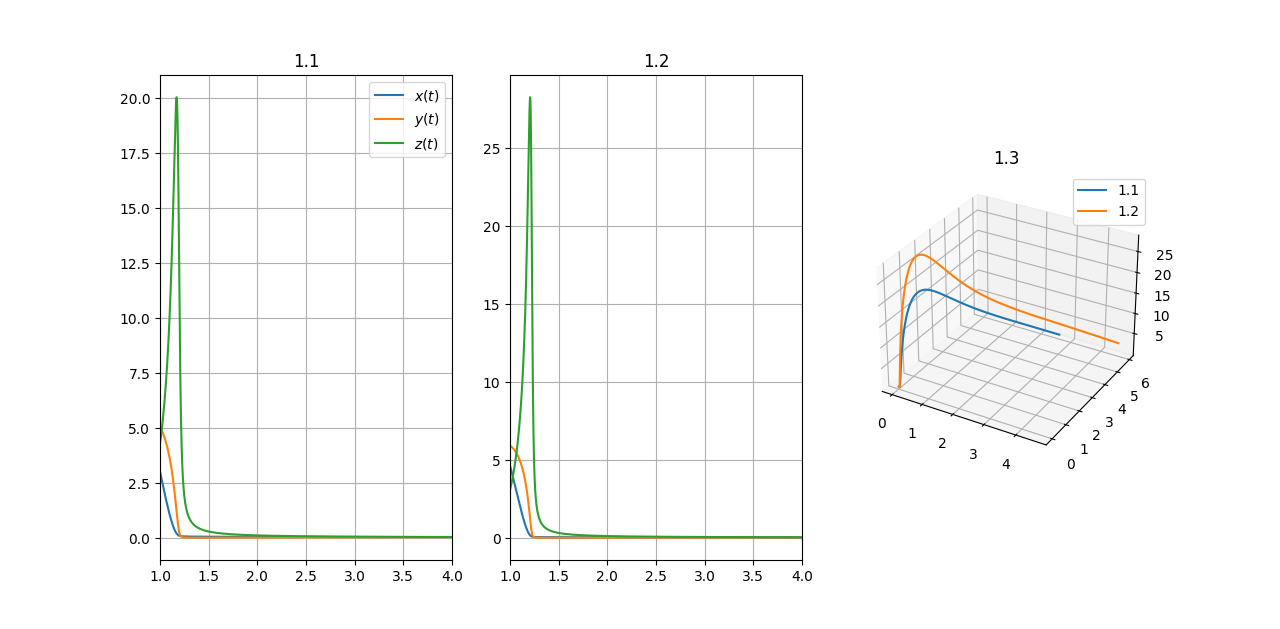
\includegraphics[width=\linewidth]{../numerical_models/images/1.png}
    \end{figure}
\end{frame}

\begin{frame}
    {Segundo experimento}

    Se usaron valores tal que $\eta > \beta$ y $\eta > \alpha$.
    $[x_0=0.3, y_0=2.4, z_0=3.9]$,
    $[x_0=0.6, y_0=2.4, z_0=3.9]$, $[x_0=2.1, y_0=1.2, z_0=1.1]$

    % La simulación muestra que todos los valores van al punto de equilibrio interior.
    \begin{figure}[h!]
        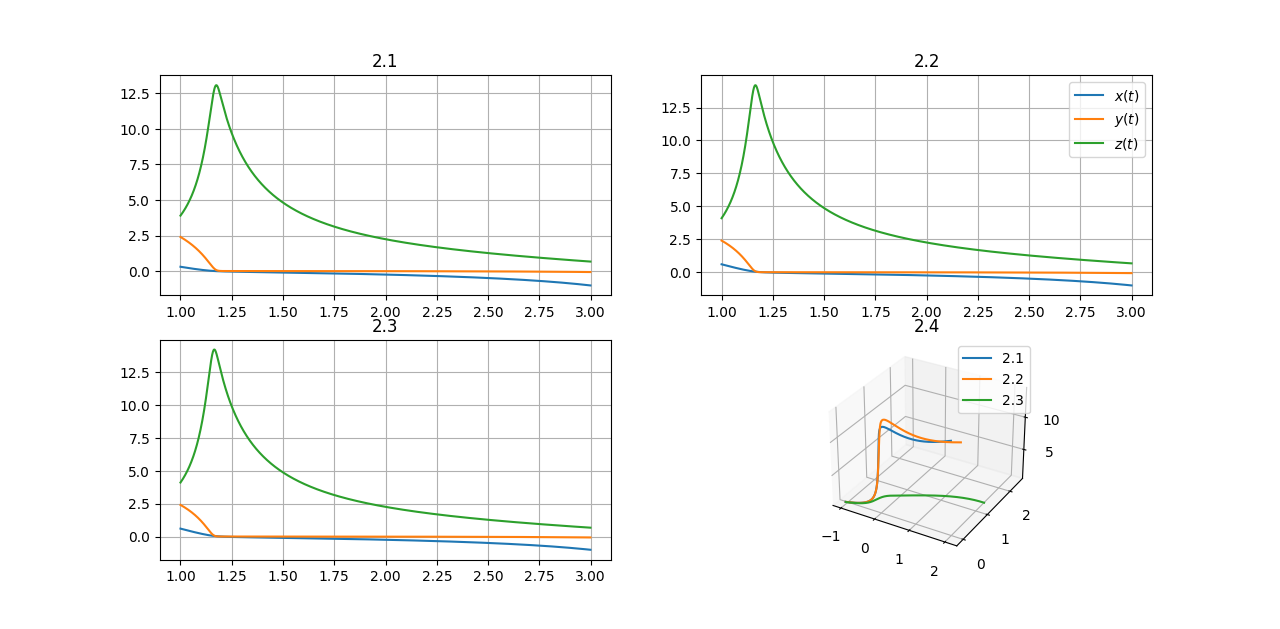
\includegraphics[width=\linewidth]{../numerical_models/images/2.png}
    \end{figure}

\end{frame}
\begin{frame}
    {Tercer experimento}

    Se usaron valores tal que $\alpha > \beta$\\
    $[x_0=0.3, y_0=2.4, z_0=3.9]$


    {\it\scriptsize Este experimento difiere del resultado dado por [1]}

    \begin{figure}[h!]
        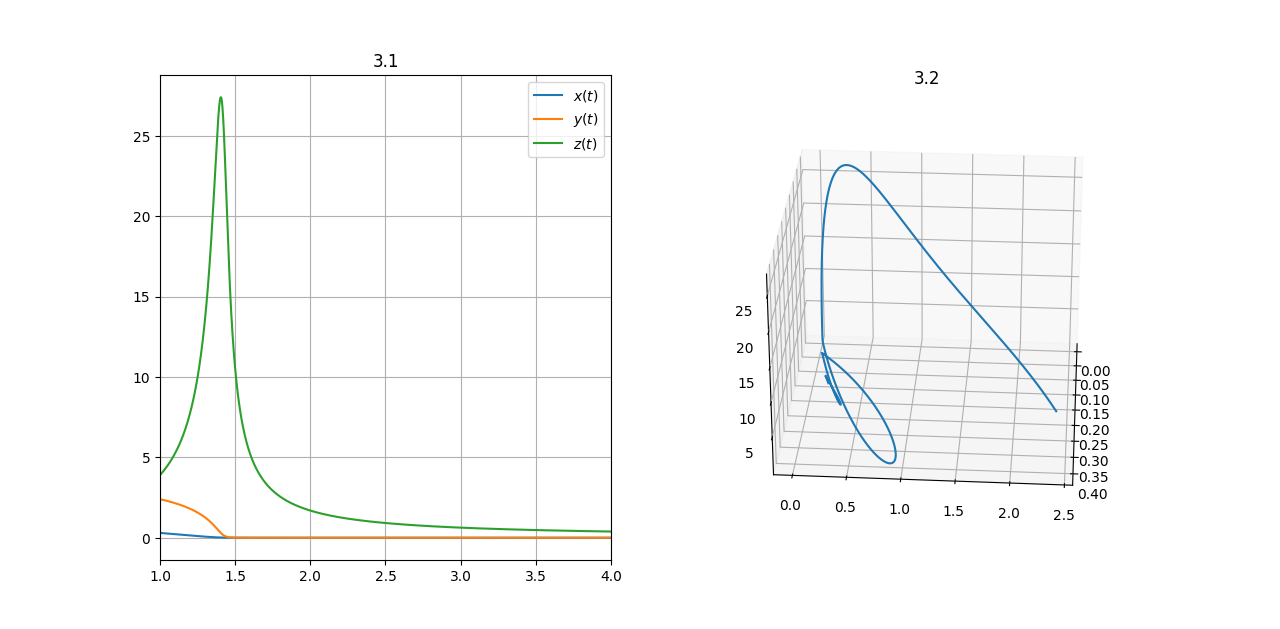
\includegraphics[width=\linewidth]{../numerical_models/images/3.png}
    \end{figure}

\end{frame}

\begin{frame}
    {Cuarto experimento}

    Se usaron valores tal que $\eta = \alpha$.\\
    $[x_0=1.2, y_0=2.1, z_0=4.28]$

    \begin{figure}[h!]
        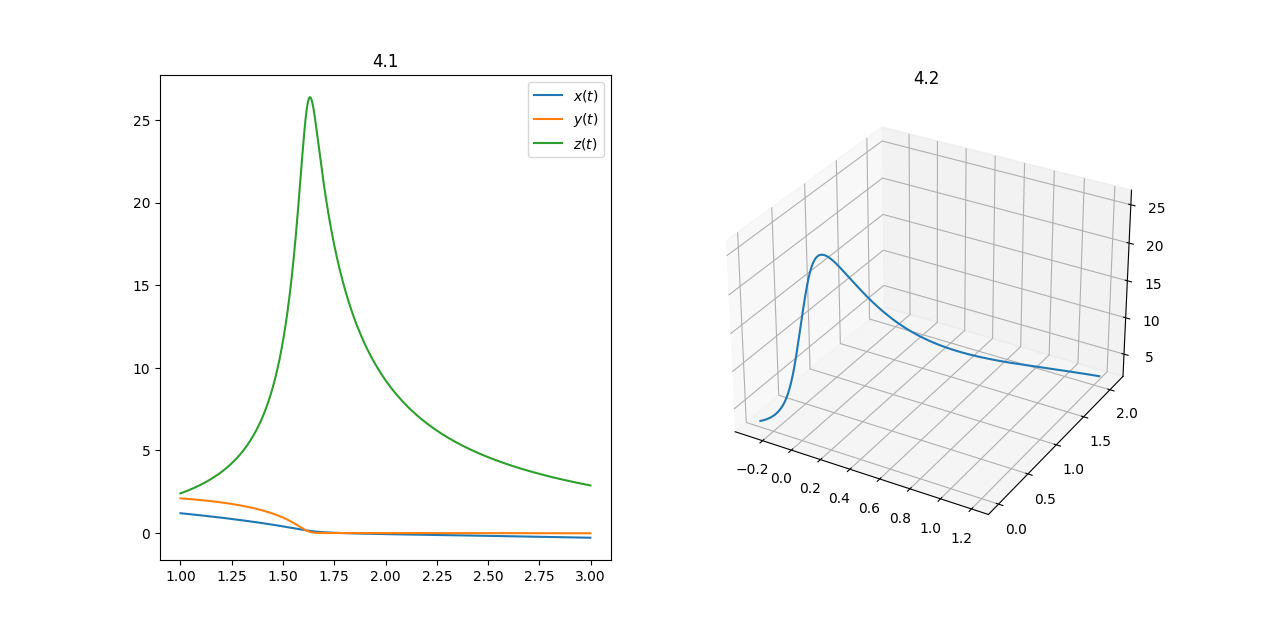
\includegraphics[width=\linewidth]{../numerical_models/images/4.png}
    \end{figure}
\end{frame}

\begin{frame}
    {Quinto experimento}

    Se usaron valores tal que $\eta > \beta$ y $\eta > \alpha$.\\
    $[x_0=1.2, y_0=2.1, z_0=2.4]$

    \begin{figure}[h!]
        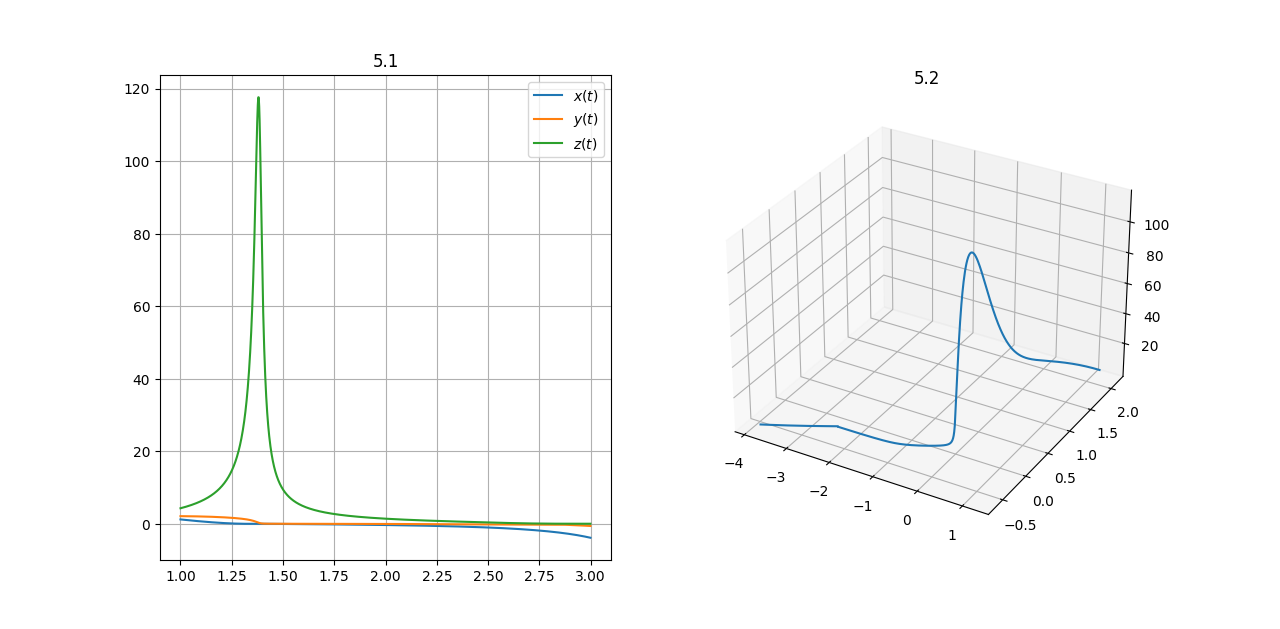
\includegraphics[width=\linewidth]{../numerical_models/images/5.png}
    \end{figure}
\end{frame}

\begin{frame}
    {Conclusiones}
    \begin{itemize}[<+->]

        \item Hemos examinado la estabilidad de un modelo de interacción presa-depredador.

        \item Se han identificado y analizado los puntos de equilibrio,
              encontrando tres equilibrios positivos:\\
              - El inicial\\
              - La extinción del depredador\\
              - Un punto interior
        \item Se ha demostrado que el punto interior es localmente estable bajo ciertas condiciones.
    \end{itemize}
\end{frame}
\begin{frame}
    {Conclusiones}
    \begin{itemize}[<+->]

        \item Las simulaciones numéricas han respaldado los resultados analíticos.

        \item Estos hallazgos contribuyen a mejorar nuestra comprensión de los sistemas ecológicos.

        \item Esta línea de trabajo podría continuar estudiando los términos que componen el modelo para lograr un mayor ajuste a la realidad de la
              naturaleza.
    \end{itemize}
\end{frame}

{ % all template changes are local to this group.
\setbeamertemplate{}{}
\begin{frame}<article:0>[plain]
    \begin{tikzpicture}[remember picture,overlay]
        \node[at=(current page.center)]{
            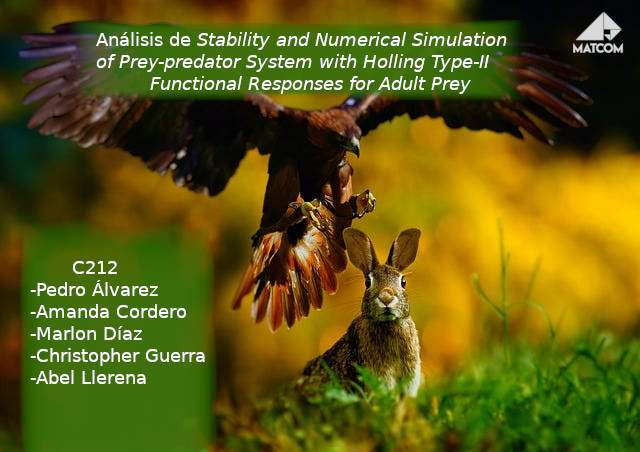
\includegraphics[width=\paperwidth,height=\paperheight]
                            {figures/present.jpg}
        };
    \end{tikzpicture}
     \end{frame}
}
\end{document}